% ===========================================================================
% SECTION 7 DISCUSSION
% Target: 600-800 words
% ===========================================================================

\section{Discussion}
\label{sec:discussion}

\subsection{Main Findings}
\label{subsec:main_findings}

Four findings emerge from this study. First, a systematic six-architecture
comparison (Section~\ref{sec:ml_surrogates}) shows that prediction accuracy
alone is a poor predictor of closed-loop usefulness: LLNFM and the two GP
variants dominate on one-step RMSE, yet PINN a mid-table predictor
achieves the best V1 closed-loop RMSE (Section~\ref{subsec:v1_results}),
while GP-v2's substantially improved open-loop accuracy over GP V1 leaves
closed-loop RMSE unchanged (Section~\ref{subsec:v1_v2_comparison}). Second,
what initially appeared to be a hard operational incompatibility between
LSTM, TCN, SW-MLP, PINN-v2, and GP-v2 on one hand and closed-loop
SQP-based \texttt{nlmpc} on the other, was traced through a five-stage
diagnostic (Section~\ref{subsec:operational_feasibility}) to a specific,
resolvable cause: repeated calls to MATLAB's \texttt{predict()} function
inside the SQP solve, not surrogate architecture, model size, or MATLAB
version. A verified manual forward pass  explicit matrix arithmetic
for feedforward and Mat\'ern-kernel architectures, and a vectorized
causal convolution for TCN  restored closed-loop viability for all
six surrogates, with speedups of $7.8\times$ to $2844\times$ and
near-elimination of real-time budget overruns
(Table~\ref{tab:predict_bypass}). This reframes what the ML-MPC-for-wind
literature would otherwise record as an architectural limitation of
deep-learning surrogates as, instead, an implementation-specific cost
that is both diagnosable and remediable within the same toolchain,
consistent with the independent report of Salzmann \emph{et al.}~\cite{salzmann_real-time_2022}
that decoupling a neural network's evaluation from the surrounding
solver's iteration loop is necessary  though not previously
documented, to our knowledge, as arising specifically from
\texttt{predict()}'s own per-call overhead in MATLAB's \texttt{nlmpc}.
A structurally related, but architecturally distinct, finding is
reported by Witter \emph{et al.}~\cite{witter_creating_2025}. Their setup contains no
predictive controller at all: an LSTM/GRU/Transformer surrogate replaces
a multibody-simulation (MBS) plant model, run in a loop with the
turbine's own standard (non-MPC) controller, rather than serving as an
MPC's internal predictive model as in this paper. Within that setup,
their LSTM/GRU surrogates 'diverge from the expected results' (their
wording) for a \emph{predictive-accuracy} reason (the learned dynamics
themselves behave differently once embedded in the feedback loop), whereas
our LSTM's closed-loop difficulty was, before the bypass,
\emph{computational} (excessive per-step latency causing the solver to
operate on a stale or default control action) rather than a divergence of
the learned dynamics  the extended Monte Carlo evaluation
(Section~\ref{subsec:monte_carlo}) shows LSTM achieving competitive, and
at some wind speeds the best, tracking accuracy once the computational
bottleneck is removed. Distinguishing these two failure modes 
functional divergence versus computational infeasibility  is
important for practitioners, since only the latter admits the kind of
implementation-level remedy demonstrated here. Third,
the Region~II/III torque switching correction
(Section~\ref{subsec:torque_switching}) while standard practice in the
classical wind turbine control literature \cite{bianchi2006,pao2009} was
in our case discovered only through long-horizon closed-loop simulation
with an incorrect constant-torque assumption; the fact that a textbook
modeling choice reproduces a documented irrecoverable failure mode
underscores that this detail cannot be treated as a minor implementation
nicety when generating training data or evaluating closed-loop MPC.
\label{subsec:gp_frozen_actuator_finding}
Fourth, applying the same diagnostic standard established by Finding 2
 explicit per-step actuator command and solver exit-flag logging,
rather than trusting an aggregate metric alone  to our own GP-based
uncertainty-penalized MPC cost (Section~\ref{subsec:gp_uncertainty_cost})
revealed that a previously reported "zero pitch activity" result, for
both GP (V1) and GP-v2 (V2), is a frozen-actuator artifact rather than a
genuine controller achievement: the pitch command never leaves its
initial value ($\text{std}=0$ across every tested step), and the solver
reports a non-positive exit flag (systematic infeasibility) at
effectively every step, independent of the uncertainty penalty weight
$\kappa$ (consistent with the inconclusive $\kappa$-sensitivity result
of Section~\ref{subsec:limitations}). This mirrors, almost exactly, the
initial-condition-driven frozen-actuator signature diagnosed in
Section~\ref{subsec:bypass_closed_loop}  identical aggregate metrics
across ostensibly different runs, here across two different GP model
generations rather than across five different architectures  and we
apply the same recognition criterion here that Section~\ref{subsec:bypass_closed_loop}
established: a report of zero actuator activity for the sole actuator
available in above-rated operation is not, on its own, evidence of good
control, and should be verified against the actuator trace and solver
status before being reported as a result. We withdraw the "zero pitch
activity" achievement claim accordingly (see
Section~\ref{subsec:limitations}) and report this finding itself, and
the general diagnostic habit that exposed it, as this paper's fourth
contribution in place of the original claim.

\begin{figure}[H]
\centering
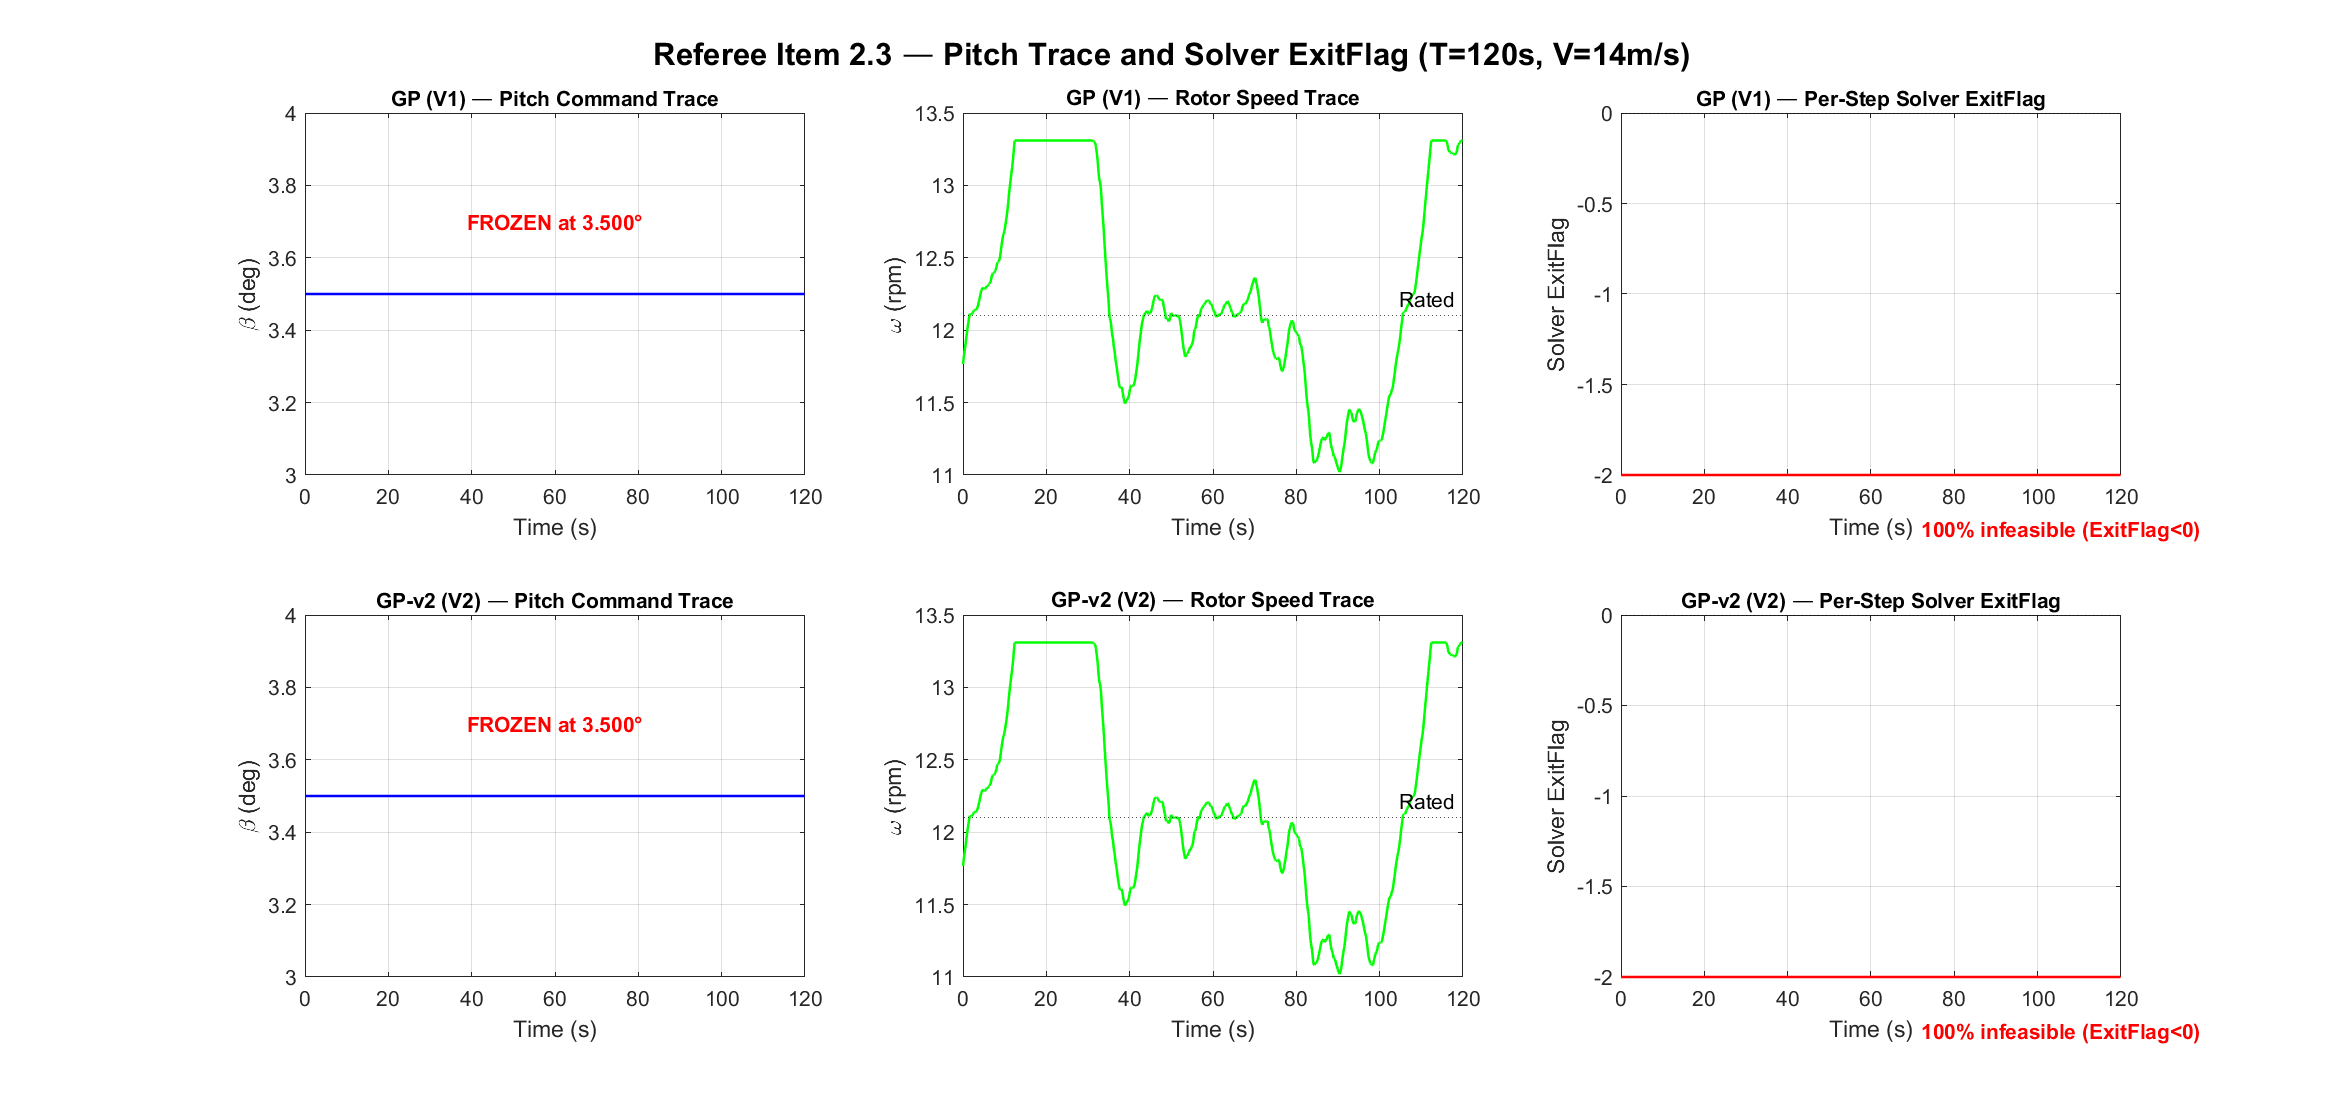
\includegraphics[width=\textwidth]{figures/FigF_GPFrozenActuator_PitchTrace.png}
\caption{Pitch command trace, rotor speed trace, and per-step solver
\texttt{ExitFlag} for GP (V1) and GP-v2 (V2) under the original
$T=\SI{120}{s}$ protocol. The pitch command is frozen at its initial
value for the full simulation in both cases ($\text{std}=0$), and
\texttt{ExitFlag}$<0$ (solver infeasibility) at every one of the
$1200$ steps tested, confirming the 'zero pitch activity' result is a
frozen-actuator artifact rather than genuine regulation.}
\label{fig:gp_frozen_actuator}
\end{figure}

Relative to the model-free reinforcement-learning alternative to
surrogate-based MPC \cite{xie_data-driven_2023}, our approach retains
MPC's explicit constraint handling and, via the manual bypass of
Section~\ref{subsec:operational_feasibility}, its real-time feasibility
argument grounded in measured per-step cost rather than only
asymptotic policy performance; a direct empirical comparison between
the two paradigms on the same plant is left to future work.

\subsection{Limitations}
\label{subsec:limitations}

Several limitations qualify these findings. The plant model retains only
two states ($\omegar,\beta$) and omits drivetrain torsion and tower
fore-aft dynamics, both of which are standard in higher-fidelity wind
turbine control models \cite{schlipf2013} and materially affect load-
relevant behavior; the reduced model is appropriate for a first
systematic surrogate comparison but likely understates the wind
turbine's dynamic order.
The wind input is spatially uniform (Section~\ref{subsec:wind_model}):
no rotational sampling or tower shadow effect is modeled, both of which
introduce periodic loading components a real turbine controller must
reject. The plant is integrated with explicit Euler at
$\Delta t=\SI{0.1}{s}$, equal to the pitch actuator time constant
$\tau_\beta$. A dedicated sensitivity check, run post hoc, confirms
this is a genuine limitation rather than the merely hypothetical
concern noted in Section~\ref{subsubsec:pinn_v1} for PINN's
degenerate residual: because $\Delta t=\tau_\beta$, Euler's discrete
pitch-actuator update reduces to $\beta_{k+1}=\beta_k+(u-\beta_k)=u$,
an instantaneous jump to the commanded pitch rather than the
$(1-e^{-1})\approx63\%$ single-time-constant approach a continuous
first-order lag would produce. Repeating a $\SI{60}{s}$
closed-loop run with the Baseline controller under classical RK4
integration of the identical continuous dynamics, instead of Euler,
leaves closed-loop RMSE essentially unchanged ($1.2709$ vs.\
$\SI{1.2734}{rpm}$, a $0.19\%$ relative difference), but cumulative
pitch activity drops by $54\%$ ($372.5$ vs.\ $\SI{172.0}{deg}$); a
follow-up variant isolating whether this arises from RK4's pitch-rate
saturation being evaluated once per integration substage (rather than
once per step, as in Euler) found the discrepancy essentially
unchanged when saturation semantics were matched to Euler's
($\SI{171.6}{deg}$), ruling out saturation handling as the cause and
confirming the Euler/$\tau_\beta$ degeneracy itself as responsible.
Because the same plant integrator underlies every controller and
surrogate reported in this paper, this bias is common across all
reported results rather than differentially favoring any one
architecture, so the \emph{relative} comparisons between controllers
that this paper's contributions rest on  computational speedup,
relative tracking accuracy, and closed-loop feasibility verdicts 
are not expected to be affected. However, cumulative pitch activity
figures reported throughout this paper (Table~\ref{tab:v1_results} and
subsequent tables) should accordingly be read as a comparative,
architecture-relative indicator rather than a physically calibrated
estimate of actuator wear; a smaller integration step decoupled from
$\tau_\beta$, noted as future work below, would be required before
absolute pitch-activity figures could be trusted on their own.
Whether the same integration artifact still explains the differing
closed-loop behavior of window-based surrogates once evaluated via the
manual bypass (Section~\ref{subsec:bypass_closed_loop}) is a related
question the present results do not settle. The
extended Monte Carlo evaluation (Section~\ref{subsec:monte_carlo}) covers
three wind speeds and five seeds each, but a single $\SI{60}{s}$ window
and no multi-objective load metric beyond rotor-speed RMSE and
cumulative pitch activity; it also surfaced an unresolved instability
(LSTM's coefficient of variation reaching $36.7\%$ at
$V=\SI{12}{m/s}$, versus $7$--$8\%$ at higher wind speeds) that this
study does not explain and that would need to be understood before
LSTM's otherwise competitive mean accuracy is trusted near the
Region~II/III boundary. The manual-bypass technique itself
(Section~\ref{subsec:operational_feasibility}) is a further limitation
in practice, not only a solution: each architecture required its own
hand-verified forward-pass implementation (layer-by-layer for
feedforward and convolutional networks, kernel-based for GP, gate
equations for LSTM), and the LSTM case specifically showed a
verification tolerance an order of magnitude looser than the other
five architectures (Table~\ref{tab:verification_tolerances} reports
the consolidated per-architecture values), attributed to single-
versus double-precision
accumulation over recurrent steps rather than a logical error but not
independently confirmed; this per-architecture verification burden does
not disappear simply because the technique is shown to work here.
The V1-to-V2 evaluation discrepancy noted for nominally unchanged
components (Persistence, LLNFM) is, as established in
Section~\ref{subsec:comparative_accuracy}, fully traced to a
deliberate widening of the V2 dataset's initial-condition sampling to
cover Region~II, not an unresolved artifact. The GP-uncertainty cost
weight $\kappa$ (Section~\ref{subsec:gp_uncertainty_cost}) is a further,
now-\emph{confirmed} limitation rather than an open question: an initial
attempt
to sweep $\kappa \in \{0, 0.2, 0.5, 0.8, 1.0\}$ under the original
\texttt{predict()}-based GP-v2 cost on a shortened $\SI{20}{s}$ window
returned a numerically identical closed-loop RMSE and zero pitch
activity for every $\kappa$ value tested, traced to
\texttt{ExitFlag}$<0$ (solver infeasibility) at every one of $200$
steps regardless of $\kappa$. A dedicated follow-up re-verification,
using the full original $\SI{120}{s}$ protocol with explicit per-step
actuator command and exit-flag logging (Section~\ref{subsec:gp_frozen_actuator_finding}),
\emph{confirms} this is not an artifact of the shortened window: both
GP (V1) and GP-v2 (V2) show the pitch command frozen at its initial
value ($\text{std}=0$) with \texttt{ExitFlag}$<0$ at all $1200$ steps
under the full protocol. This echoes, in a more severe form, the
systematic
non-convergence under \texttt{MaxIterations}$=30$ documented for
GP-v2 in the Jacobian test of Section~\ref{subsec:operational_feasibility}
(Stage 3): there, the solver failed to converge to optimality but still
produced a moving, feasible control trajectory; here, under the
uncertainty-penalized cost specifically, the solver cannot find a
feasible solution at all. The uncertainty-penalized GP cost formulation
of Section~\ref{subsec:gp_uncertainty_cost} is accordingly not usable
in its current form, and the "zero pitch activity" result reported for
it is withdrawn (Section~\ref{subsec:gp_frozen_actuator_finding}) rather
than reported as a finding. A separate limitation, whose full picture changed materially over the
course of this investigation, concerns the $N_c=1$ control horizon used
throughout the V2 protocol. Under an earlier, since-corrected torque-law
calibration (Section~\ref{subsec:torque_switching}), PINN-v2 and TCN were
found to produce numerically identical closed-loop results across all
$15$ wind-speed/seed combinations of the extended Monte Carlo evaluation
(Section~\ref{subsec:monte_carlo}). Code inspection ruled out a software
bug (the two controllers are built and dispatched via entirely
independent code paths), and a follow-up test at $N_c=4$ under that same
torque calibration indicated the identity was a genuine corner-solution
coincidence: TCN's result was virtually unchanged between $N_c=1$ and
$N_c=4$, while PINN-v2's activity increased substantially, suggesting
PINN-v2's $N_c=1$ passivity was a control-horizon artifact and TCN's was
a genuine, $N_c$-independent property.\\ \textbf{This TCN conclusion did
not survive adoption of the corrected, NREL-reference torque-switching
parameters} (Section~\ref{subsec:torque_switching}): re-running the
identical $N_c=1$ protocol under the corrected physics, TCN no longer
matches PINN-v2 at all and instead shows substantial, unremarkable pitch
activity ($\text{PA}=\SI{272.7}{deg}$, comparable to Baseline's
$\SI{299.7}{deg}$), while PINN-v2's passivity persists unchanged
($\text{PA}=\SI{2.7}{deg}$, identical to its pre-correction value). We
therefore withdraw the specific claim that TCN's low activity is a
genuine, $N_c$-independent architectural property  it now appears to
have been a coincidence of the earlier, miscalibrated torque law, not a
property of TCN itself. PINN-v2's passivity, by contrast, reproduces
identically across both torque-law calibrations, which is more
consistent with (though does not by itself prove) a genuine
architecture-driven local optimum. The original $N_c=4$ comparison was
run only under the pre-correction torque law and has not yet been
repeated under the corrected physics; consequently, whether PINN-v2's
passivity would likewise open up under $N_c=4$ with the corrected
torque law is an open question, not a settled one, and is flagged for
the next verification pass rather than assumed. More broadly, this
episode is itself a useful illustration of the diagnostic standard this
paper applies throughout: a finding that appeared solid under one set of
physical parameters did not survive a subsequent, independently
motivated correction to those parameters, and is reported as withdrawn
rather than left uncorrected. $N_c=1$ closed-loop results for any single
surrogate should not be assumed representative of that surrogate's
behavior under a less constrained horizon without independent
verification under the currently adopted plant parameters. Finally, prediction and tracking accuracy
are reported throughout this paper as RMSE alone; MAE and $R^2$ were
not computed retroactively for already-reported results, since doing
so would require the original per-sample prediction arrays rather than
the aggregate RMSE values actually logged during each run  a
utility function (\texttt{compute\_extended\_metrics.m}) is provided
for future evaluation runs to report all three metrics jointly,
avoiding a repeat of this retroactive gap.

\subsection{Threats to Validity}
\label{subsec:threats_to_validity}

\textbf{Non-convergence.} Every controller in this paper operates under
a bounded $30$-iteration SQP budget, and \texttt{ExitFlag} is
non-positive at effectively every step for every controller, including
the well-behaved Baseline (Appendix~\ref{subsec:appendix_exitflag}). A
sensitivity sweep over the iteration cap (Baseline, TCN, MLP-residual;
$10$--$100$ iterations) tests directly whether this materially affects
reported results.

\textbf{Single toolchain.} Every result in this paper comes from a
single software ecosystem (MATLAB, Deep Learning Toolbox), tested
across two releases (R2024a, R2026a) but with no cross-toolchain
replication (e.g.\ Python/PyTorch + CasADi/acados). The
\texttt{predict()}-overhead finding is not claimed to generalize beyond
this specific toolchain.

\textbf{Two-state plant.} The reduced rotor-speed/pitch model omits
drivetrain torsion and tower fore-aft dynamics; load-relevant
conclusions should not be drawn from this study without validation on
a higher-order model.

\textbf{Five-seed sample.} The extended Monte Carlo evaluation uses
five wind seeds per condition -- sufficient to characterize gross
trends (e.g.\ LSTM's instability at $V=\SI{12}{m/s}$) but too few for
tight confidence intervals on any single controller's mean performance.

\textbf{No significance testing.} Comparisons between controllers
throughout this paper (e.g.\ Table~\ref{tab:monte_carlo_extended})
report mean $\pm$ standard deviation without formal hypothesis
testing (e.g.\ paired $t$-tests or a non-parametric equivalent across
matched wind seeds). Apparent differences between controllers should be
read as descriptive, not as statistically established.

\subsection{Perspectives (V3)}
\label{subsec:perspectives_v3}

Five directions follow from the findings above. First, the LSTM
instability at $V=\SI{12}{m/s}$ (Section~\ref{subsec:monte_carlo}) and
the crossover in wind-speed sensitivity between
Baseline/GP/residual-MLP/SW-MLP and PINN-v2/TCN
(Section~\ref{subsec:monte_carlo}) both warrant targeted investigation
 extending the wind-speed sweep beyond three points and pairing it
with the multi-objective load metrics noted above would clarify whether
these are genuine architectural properties or artifacts of the specific
training data distribution. Second, extending the plant to four states
by adding drivetrain torsion and tower fore-aft dynamics
\cite{schlipf2013} would let the comparison generalize to
load-relevant metrics, not only rotor-speed tracking, and would provide
a further, independent test of whether the manual-bypass technique
scales to a higher-order plant and correspondingly larger surrogates.
Third, decoupling the plant integration step from the pitch actuator
time constant ($\Delta t \ne \tau_\beta$, e.g.\ via RK4 integration or
a smaller $\Delta t$ with actuator sub-stepping) would remove the
Euler/$\tau_\beta$ degeneracy identified above and allow the cumulative
pitch-activity figures reported throughout this paper to be
re-evaluated as physically calibrated actuator-wear estimates, rather
than only architecture-relative comparisons. Fourth, an explicit
wind-speed forecasting or estimation layer an
autoregressive predictor over the MPC horizon, or an Extended Kalman
Filter estimating rotor-effective wind speed from standard turbine
measurements \cite{soltani2013} would let the controller anticipate
disturbances rather than react to the current measured $V$ alone, and
is a natural complement to a repaired GP uncertainty-penalized cost
formulation, should one be developed (see below).
Fifth, and directly motivated
by the confirmed frozen-actuator finding above
(Section~\ref{subsec:gp_frozen_actuator_finding}), diagnosing
\emph{why} the GP-uncertainty-penalized cost drives the SQP solver to
infeasibility independent of $\kappa$'s value whether through
supplying an analytical (rather than finite-difference) Jacobian for
\texttt{cost\_gp.m} specifically, relaxing the control horizon
$N_c=1$ constraint identified as a contributing factor in the Stage~3
Jacobian test, or reformulating the uncertainty term as a tightened
constraint rather than a cost penalty (in the spirit of
the probabilistic reachable sets of Hewing \emph{et al.}~\cite{hewing2020}) is a prerequisite
for any future uncertainty-penalized GP-MPC cost on this plant, since
the present formulation is withdrawn rather than merely unvalidated.
A structurally different route to the same real-time
feasibility goal, not explored in this paper, would replace the
nonlinear surrogate entirely with a Koopman-operator-based linear
approximation \cite{williams2015}, trading the accuracy of a
nonlinear model for the computational simplicity of linear MPC.
Coupling the corrected two-state
model to a higher-fidelity aeroelastic code (e.g.\ OpenFAST) is a longer-
term validation step once these nearer-term extensions are in place.
